%%%%%%%%%%%%%%%%%%%%%%%%%%%%%%%%%%%%%%%%%%%%%%%%%%%%%%%%%%%%%%%%%%%%%%%%%%%%%%%%%%%%%%%%%%%%%%%%%%%%%%%%%%%%%%%%
%%%%%%%%%%%%%%%%%%%%%%%%%%%%%%%%%%%%%%%%%%%%%% VARIABLEN %%%%%%%%%%%%%%%%%%%%%%%%%%%%%%%%%%%%%%%%%%%%%%%%%%%%%%%
%%%%%%%%%%%%%%%%%%%%%%%%%%%%%%%%%%%%%%%%%%%%%%%%%%%%%%%%%%%%%%%%%%%%%%%%%%%%%%%%%%%%%%%%%%%%%%%%%%%%%%%%%%%%%%%%

\newcommand{\Autor}					{Sebastian H{\"u}ther \& Lorenzo Toso}
\newcommand{\Matrikelnummer}		{8853105 \& 1906813}
\newcommand{\Kurs}					{TINF12B3}
\newcommand{\Studienfach}			{Informationstechnik}
\newcommand{\Ausbildungsfirma}		{Karlsruher Institut f\"ur Technologie}
\newcommand{\Universitaet}			{DHBW Karlsruhe}
\newcommand{\Betreuer}				{Gertrud Nieder}

\newcommand{\Bearbeitungszeitraum}	{2 Semester}
\newcommand{\Berichttyp}			{Studienarbeit}
\newcommand{\Datum}					{\today}
\newcommand{\Titel}					{Gegenstandserkennung und kategoriebasierter Transport anhand von
kameraunterst\"utzten NXT-Robotern}

\newcommand{\Schriftgroesse}		{12pt}
\newcommand{\Zeilenabstand}			{1.5}
\newcommand{\LinkerRand}			{25mm}
\newcommand{\RechterRand}			{25mm}
\newcommand{\ObererRand}			{25mm}
\newcommand{\UntererRand}			{25mm}



%%%%%%%%%%%%%%%%%%%%%%%%%%%%%%%%%%%%%%%%%%%%%%%%%%%%%%%%%%%%%%%%%%%%%%%%%%%%%%%%%%%%%%%%%%%%%%%%%%%%%%%%%%%%%%%%
%%%%%%%%%%%%%%%%%%%%%%%%%%%%%%%%%%%%%%%%%%%%%% DO NOT TOUCH %%%%%%%%%%%%%%%%%%%%%%%%%%%%%%%%%%%%%%%%%%%%%%%%%%%%
%%%%%%%%%%%%%%%%%%%%%%%%%%%%%%%%%%%%%%%%%%%%%%%%%%%%%%%%%%%%%%%%%%%%%%%%%%%%%%%%%%%%%%%%%%%%%%%%%%%%%%%%%%%%%%%%


\documentclass[	\Schriftgroesse,							%Schriftgröße
								listof=totoc,										%Abbildungs und Tabellenverzeichnis im Inhaltsverzeichnis
								bibliography=totoc,											%Literaturverzeichnis ins Inhaltsverzeichnis
								a4paper,
								] {scrreprt}



\usepackage[dvipdfm]{geometry}
\usepackage{fancyhdr}														% Kopf und Fußzeile
\usepackage[T1]{fontenc}													% Schriftart	
\usepackage[utf8]{inputenc}													% Umlaute
\usepackage[ngerman]{babel}													% Deutsche Silbentrennung
\usepackage{mathptmx}														% Schriftart
\usepackage[printonlyused]{acronym}											% Abkuerzungsverzeichnis
\usepackage{graphicx}														% Bilder einfügen
\usepackage{ifthen}															% ifabfragen
\usepackage{calc}															% einfache Rechnungen
\usepackage{SIunits}														% Einheiten wie micro etc
\usepackage{titlesec}														% Um Chapterseiten nen Style zuzuweisen
\usepackage{geometry}														% LAYOUT
\hbadness=10000 															% ignore underfull boxes
\usepackage[numbers,sort]{natbib}											% Literaturverzeichnis
\usepackage[pdftex,
			bookmarks=true, 
			pdftitle={\Titel}, 
			pdfauthor={\Autor}
			]{hyperref}														% Links
\usepackage{blindtext}														% Zu test zwecken

\usepackage{zahl2string} 													% Um Zahlen in Strings zu wandeln 2 -> zwei
\usepackage{tabularx}														% Tabellen auf Seitenbreite anpassen

\usepackage[Algorithmus]{algorithm} 										% Algorithmen beschriften/durchnummerieren etc
\usepackage{algpseudocode} 													% Pseudocode

\usepackage{amsmath} 														% Gleichungen an Gleichheitszeichen ausrichten
\usepackage{comment}														% Um für QUICKPRINT alles auszukommentieren

\usepackage{multirow}														% \multirow in Tabellen
\usepackage{booktabs}														% Schönere Tabellenstriche
\usepackage[format=plain, justification=centering]{caption}											% Schönere Bildunterschriften

% \todo Notizen
\usepackage[enable]{easy-todo}

% \enquote "..."
\usepackage{csquotes}

% JAVA LISTINGS
\usepackage{listings}
\usepackage{color}

\definecolor{pblue}{rgb}{0.13,0.13,1}
\definecolor{pgreen}{rgb}{0,0.5,0}
\definecolor{pred}{rgb}{0.9,0,0}
\definecolor{pgrey}{rgb}{0.46,0.45,0.48}
\lstset{language=Java,
  basicstyle=\footnotesize,
  frame=L,
  showspaces=false,
  showtabs=false,
  breaklines=true,
  showstringspaces=false,
  breakatwhitespace=true,
  commentstyle=\color{pgreen},
  keywordstyle=\color{pblue},
  stringstyle=\color{pred},
}


%%%%%%%%%%%%%%%%%%%%%%%%%%%%%%%%%%%%%%%%%%%%%%%%%%%%%%%%%%%%%%%%%%%%%%%%%%%%%%%%%%%%%%%%%%%%%%%%%%%%%%%%%%%%%%%%
%%%%%%%%%%%%%%%%%%%%%%%%%%%%%%%%%%%%%%%%%%%%%% TEST BOOLS %%%%%%%%%%%%%%%%%%%%%%%%%%%%%%%%%%%%%%%%%%%%%%%%%%%%%%
%%%%%%%%%%%%%%%%%%%%%%%%%%%%%%%%%%%%%%%%%%%%%%%%%%%%%%%%%%%%%%%%%%%%%%%%%%%%%%%%%%%%%%%%%%%%%%%%%%%%%%%%%%%%%%%%



\newboolean{QUICK}						\setboolean{QUICK}							{false}
\newboolean{PRINT}						\setboolean{PRINT}							{false}
\newboolean{FULL}						\setboolean{FULL}							{false}



\newboolean{ShowTODO}					\setboolean{ShowTODO}						{false}
\newboolean{RomanNumbering}				\setboolean{RomanNumbering}					{true}
\newboolean{ShowSubSectionsInTOC}		\setboolean{ShowSubSectionsInTOC}			{false}
\newboolean{Layouted}					\setboolean{Layouted}						{true}
\newboolean{Images}						\setboolean{Images}							{true}
\newboolean{Tables}						\setboolean{Tables}							{true}
\newboolean{Equations}					\setboolean{Equations}						{true}

\newboolean{Titelseite}					\setboolean{Titelseite}						{true}
\newboolean{Inhaltsverzeichnis}			\setboolean{Inhaltsverzeichnis}				{true}
\newboolean{EidesstattlicheErklaerung}	\setboolean{EidesstattlicheErklaerung}		{true}
\newboolean{Chapters}					\setboolean{Chapters}						{true}
\newboolean{Abkuerzungsverzeichnis}		\setboolean{Abkuerzungsverzeichnis}			{false}
\newboolean{Abbildungsverzeichnis}		\setboolean{Abbildungsverzeichnis}			{true}
\newboolean{Literaturverzeichnis}		\setboolean{Literaturverzeichnis}			{true}
\newboolean{DeadChapters}				\setboolean{DeadChapters}					{false}



%%%%%%%%%%%%%%%%%%%%%%%%%%%%%%%%%%%%%%%%%%%%%%%%%%%%%%%%%%%%%%%%%%%%%%%%%%%%%%%%%%%%%%%%%%%%%%%%%%%%%%%%%%%%%%%%
%%%%%%%%%%%%%%%%%%%%%%%%%%%%%%%%%%%%%%%%%%%%%% AUTOMATIC LAYOUT %%%%%%%%%%%%%%%%%%%%%%%%%%%%%%%%%%%%%%%%%%%%%%%%
%%%%%%%%%%%%%%%%%%%%%%%%%%%%%%%%%%%%%%%%%%%%%%%%%%%%%%%%%%%%%%%%%%%%%%%%%%%%%%%%%%%%%%%%%%%%%%%%%%%%%%%%%%%%%%%%
\geometry
{
left=\LinkerRand,
right=\RechterRand,
top=\ObererRand,
bottom=\UntererRand,
includehead,
includefoot,
%showframe,
}


%%%%%%%%%%%%%%%%%%%%%%%%%%%%%%%%%%%%%%%%%%%%%%%%%%%%%%%%%%%%%%%%%%%%%%%%%%%%%%%%%%%%%%%%%%%%%%%%%%%%%%%%%%%%%%%%
%%%%%%%%%%%%%%%%%%%%%%%%%%%%%%%%%%%%%%%%%%%%%% HEADER AND FOOTER %%%%%%%%%%%%%%%%%%%%%%%%%%%%%%%%%%%%%%%%%%%%%%%
%%%%%%%%%%%%%%%%%%%%%%%%%%%%%%%%%%%%%%%%%%%%%%%%%%%%%%%%%%%%%%%%%%%%%%%%%%%%%%%%%%%%%%%%%%%%%%%%%%%%%%%%%%%%%%%%

\pagestyle{fancy}
\fancyhead[R]{\thepage}
\fancyhead[L]{\leftmark}
\fancyfoot[C]{}
\fancyfoot[R]{\Universitaet}
\fancyfoot[L]{\Autor}
\renewcommand{\headrulewidth}{0.4pt}
\renewcommand{\footrulewidth}{0.4pt}
\renewcommand{\thefootnote}{\arabic{footnote}}
%Formatierung der Kapitelüberschrift für Kopf- und Fußzeile
\renewcommand{\chaptermark}[1]{ \markboth{\textsc{\chaptername}\ \thechapter\hspace{0.4cm}--\hspace{0.4cm}#1}{}}


%%%%%%%%%%%%%%%%%%%%%%%%%%%%%%%%%%%%%%%%%%%%%%%%%%%%%%%%%%%%%%%%%%%%%%%%%%%%%%%%%%%%%%%%%%%%%%%%%%%%%%%%%%%%%%%%
%%%%%%%%%%%%%%%%%%%%%%%%%%%%%%%%%%%%%%%%%%%%%% OTHER OPTIONS %%%%%%%%%%%%%%%%%%%%%%%%%%%%%%%%%%%%%%%%%%%%%%%%%%%
%%%%%%%%%%%%%%%%%%%%%%%%%%%%%%%%%%%%%%%%%%%%%%%%%%%%%%%%%%%%%%%%%%%%%%%%%%%%%%%%%%%%%%%%%%%%%%%%%%%%%%%%%%%%%%%%

\author{\Autor}
\date{	\Datum}
\title{	\Titel}

\newcounter{my-temp-counter}
\newcounter{tempCount}
\newcounter{tempCount2}
\newcommand{\chapNoToTextRef}[1]{\setcounterref{my-temp-counter}{#1}\hyperref[#1]{\numstring{my-temp-counter}}} % Kapitel verweis ausgeschrieben

\setlength{\parindent}{0cm}																						% Keine Abstand bei neuem Absatz
\renewcommand{\baselinestretch}{\Zeilenabstand}																	% Zeilenabstand
\renewcommand*{\chapterheadstartvskip}{\vspace*{-5mm}}															%ABSTAND VOR CHAPTER VERRINGERN

\assignpagestyle{\chapter}{fancy}																				% Chapterseiten auch Stylen
\setlength{\parskip}{10pt}																						% Absatzhöhe


\clubpenalty 			= 10000 
\widowpenalty 			= 10000 																				% Schusterjungen und Hurenkinder vermeiden 
\displaywidowpenalty 	= 10000


\ifthenelse{\boolean{QUICK}}
{
		\setboolean{PRINT}												{false}
		
		\setboolean{ShowTODO}											{false}
		\setboolean{RomanNumbering}										{false}
		\setboolean{ShowSubSectionsInTOC}								{false}
		\setboolean{Layouted}											{false}
		\setboolean{Images}												{false}
		\setboolean{Tables}												{false}
		\setboolean{Equations}											{false}
		
		\setboolean{Titelseite}											{false}
		\setboolean{Inhaltsverzeichnis}									{false}
		\setboolean{EidesstattlicheErklaerung}							{false}
		\setboolean{Chapters}											{true}
		\setboolean{Abkuerzungsverzeichnis}								{false}
		\setboolean{Abbildungsverzeichnis}								{false}
		\setboolean{Literaturverzeichnis}								{false}
		\setboolean{DeadChapters}										{false}
}{}
\ifthenelse{\boolean{PRINT}}
{
		\setboolean{QUICK}												{false}
		
		\setboolean{ShowTODO}											{false}
		\setboolean{RomanNumbering}										{false}
		\setboolean{ShowSubSectionsInTOC}								{true}
		\setboolean{Layouted}											{true}
		\setboolean{Images}												{true}
		\setboolean{Tables}												{true}
		\setboolean{Equations}											{true}

		\setboolean{Titelseite}											{true}
		\setboolean{Inhaltsverzeichnis}									{true}
		\setboolean{EidesstattlicheErklaerung}							{true}
		\setboolean{Chapters}											{true}
		\setboolean{Abkuerzungsverzeichnis}								{true}
		\setboolean{Abbildungsverzeichnis}								{true}
		\setboolean{Literaturverzeichnis}								{true}
		\setboolean{DeadChapters}										{false}
}{}
\ifthenelse{\boolean{FULL}}
{
		\setboolean{QUICK}												{true}
		
		\setboolean{ShowTODO}											{true}
		\setboolean{RomanNumbering}										{true}
		\setboolean{ShowSubSectionsInTOC}								{true}
		\setboolean{Layouted}											{true}
		\setboolean{Images}												{true}
		\setboolean{Tables}												{true}
		\setboolean{Equations}											{true}
		
		\setboolean{Titelseite}											{true}
		\setboolean{Inhaltsverzeichnis}									{true}
		\setboolean{EidesstattlicheErklaerung}							{true}
		\setboolean{Chapters}											{true}
		\setboolean{Abkuerzungsverzeichnis}								{true}
		\setboolean{Abbildungsverzeichnis}								{true}
		\setboolean{Literaturverzeichnis}								{true}
		\setboolean{DeadChapters}										{true}
}{}


\ifthenelse{\boolean{ShowSubSectionsInTOC}}
{}{
		\setcounter{tocdepth}{1}		%HIDE SUBSECTIONS
}
\ifthenelse{\boolean{Images}}{}
{
	\excludecomment{figure}
	\let\endfigure\relax
	\renewcommand{\includegraphics}[2][]{}
}
\ifthenelse{\boolean{Tables}}{}
{
	\excludecomment{table}
	\let\endtable\relax
}
\ifthenelse{\boolean{Tables}}{}
{
	\excludecomment{equation}
	\let\endequation\relax
}
\ifthenelse{\boolean{Layouted}}{}
{
	\renewcommand{\newpage}{}
	\renewcommand{\samepage}{}
	\renewcommand{\vspace}{}
}

%%%%%%%%%%%%%%%%%%%%%%%%%%%%%%%%%%%%%%%%%%%%%%%%%%%%%%%%%%%%%%%%%%%%%%%%%%%%%%%%%%%%%%%%%%%%%%%%%%%%%%%%%%%%%%%%
%%%%%%%%%%%%%%%%%%%%%%%%%%%%%%%%%%%%%%%%%%%%%% SILBENTRENNUNG %%%%%%%%%%%%%%%%%%%%%%%%%%%%%%%%%%%%%%%%%%%%%%%%%%
%%%%%%%%%%%%%%%%%%%%%%%%%%%%%%%%%%%%%%%%%%%%%%%%%%%%%%%%%%%%%%%%%%%%%%%%%%%%%%%%%%%%%%%%%%%%%%%%%%%%%%%%%%%%%%%%
\hyphenation{Re-kon-struk-tion}
\hyphenation{Mi-kro-skop}
\hyphenation{Gauß-e-li-mi-na-tion}
\hyphenation{Spei-cher-ein-spar-ung}
\hyphenation{schluss-end-lich}
\hyphenation{LEGO}



%%%%%%%%%%%%%%%%%%%%%%%%%%%%%%%%%%%%%%%%%%%%%%%%%%%%%%%%%%%%%%%%%%%%%%%%%%%%%%%%%%%%%%%%%%%%%%%%%%%%%%%%%%%%%%%%
%%%%%%%%%%%%%%%%%%%%%%%%%%%%%%%%%%%%%%%%%%%%%%%%%%%% COMMANDS %%%%%%%%%%%%%%%%%%%%%%%%%%%%%%%%%%%%%%%%%%%%%%%%%%
%%%%%%%%%%%%%%%%%%%%%%%%%%%%%%%%%%%%%%%%%%%%%%%%%%%%%%%%%%%%%%%%%%%%%%%%%%%%%%%%%%%%%%%%%%%%%%%%%%%%%%%%%%%%%%%%
\newcommand{\np}{\par}
%\bigskip}
%\newcommand{\nl}{\par\medskip}
\newcommand{\usableWidth}	{\paperwidth-\LinkerRand-\RechterRand}
\newcommand{\usableHeight}{\paperheight-\ObererRand-\UntererRand}
\newcommand{\useAcronym}[1]{\vphantom{\ac{#1}}}
%\renewcommand{\newpage}{\ifthenelse{\boolean{Layouted}}{\newpage}{}}
\newcommand{\skl}{\langle}
\newcommand{\skr}{\rangle}

%%%%%%%%%%%%%%%%%%%%%%%%%%%%%%%%%%%%%%%%%%%%%%%%%%%%%%%%%%%%%%%%%%%%%%%%%%%%%%%%%%%%%%%%%%%%%%%%%%%%%%%%%%%%%%%%
%%%%%%%%%%%%%%%%%%%%%%%%%%%%%%%%%%%%%%%%%%%%%%%%%%%% DOKUMENT %%%%%%%%%%%%%%%%%%%%%%%%%%%%%%%%%%%%%%%%%%%%%%%%%%
%%%%%%%%%%%%%%%%%%%%%%%%%%%%%%%%%%%%%%%%%%%%%%%%%%%%%%%%%%%%%%%%%%%%%%%%%%%%%%%%%%%%%%%%%%%%%%%%%%%%%%%%%%%%%%%%
\begin{document}          
	
	\ifthenelse{\boolean{RomanNumbering}}
	{
		\pagenumbering{Roman} 
	}
	{
		\pagenumbering{arabic} 
	}
	
	\ifthenelse{\boolean{Titelseite}}
	{
		\begin{titlepage}


	\setlength{\hoffset}{ (\RechterRand-\LinkerRand)/2 }								% Titelseite zentrieren
	
	\begin{centering}
	
    
\includegraphics[width=5cm]{Bilder/Titelseite/KIT-Logo}						%KIT LOGO
		\hfill																														% Platz nach rechts
    
\includegraphics[width=5cm]{Bilder/Titelseite/DHBW-Logo}					%DHBW LOGO
		\vspace{2.5cm}																										%Platz nach unten
		
		
		\textbf{\LARGE{\Titel}}		\vspace{.7cm}\\
		\Berichttyp \vspace{.7cm}\\
		für die Prüfung zum\\
		Bachelor of Engineering\vspace{1cm}\\
		von\\
		\Autor\vspace{.2cm}\\
		\Datum
		
		\vfill
		
		\begin{tabular}{ll}
			\textbf{ Bearbeitungszeitraum:	}	&	\Bearbeitungszeitraum					\vspace{0.2cm}			\\
			\textbf{ Matrikelnummer:		}	&	\Matrikelnummer							\vspace{0.2cm}			\\
			\textbf{ Kurs:					}	&	\Kurs									\vspace{0.2cm}			\\
			\textbf{ Studienfach:			}	&	\Studienfach									\vspace{0.2cm}			\\
			\textbf{ Ausbildungsfirma:		}	&	\Ausbildungsfirma						\vspace{0.2cm}			\\
			\textbf{ Betreuer: 				}	&	\Betreuer								\vspace{0.2cm}			\\
		\end{tabular}
	\end{centering}
\end{titlepage}


	}{}
	
	\ifthenelse{\boolean{EidesstattlicheErklaerung}}
	{
		\fancyhead[L]{Eidesstattliche Erklärung}
			\newpage

\addcontentsline{toc}{chapter}{Eidesstattliche Erklärung}					% IN Inhaltsverzeichnis
\vspace*{\fill}																% Vertikal Zentrieren

{

\begin{center}
	\huge {\bf Eidesstattliche Erklärung}
	\label{cha:eidesstattlicheErklaerung}
\end{center}

\vspace{2cm}

Gemäß § 5 (3) der „Studien- und Prüfungsordnung DHBW Technik“ vom 22. September 2011.\\
Ich habe die vorliegende Arbeit selbstständig verfasst und keine anderen als die angegebenen 
Quellen und Hilfsmittel verwendet. \\
\vspace{2cm}


\begin{table}[h]
%	\centering
		\begin{tabular}{ll}
\rule{6.5cm}{0.3pt} & \rule{6.5cm}{0.3pt}\\
Ort, Datum  & Unterschrift\\
		\end{tabular}
\end{table}

}

\vspace*{\fill}
\newpage
		\fancyhead[L]{\leftmark}
	}{}
	
%	\fancyhead[L]{Abstract}
	\chapter*{Abstract}
\addcontentsline{toc}{chapter}{Abstract}

In dieser Studienarbeit wurde ein Robotersystem entwickelt, dessen Ziel es ist kameragestützt Objekte zu erkennen. Der Roboter fährt die Gegenstände an, kategorisiert diese und transportiert sie abhängig von der Kategorisierung in eine Zielzone. Für die Realisierung wurde ein Lego Mindstorms NXT Roboter und ein Google Nexus 5 Smartphone verwendet. Die Objekterkennung wurde mit bekannten Verfahren aus der Bildverarbeitung mit Hilfe der OpenCV-Bilbiothek implementiert. Der Roboter orientiert sich im Raum mit Hilfe einer Positionsverfolgung über die gefahrene Strecke. Unter Verwendung dieser Methoden konnte ein System entworfen werden, welches einen Gegenstand in weniger als einer Minute verräumen kann.

In this ...
%	\fancyhead[L]{\leftmark}
	
	\ifthenelse{\boolean{Inhaltsverzeichnis}}
	{
		\tableofcontents
\label{cha:inhalt}
	}{}
	
	
	
	\ifthenelse{\boolean{RomanNumbering}}
	{
		\newcount\romannumber
		\romannumber=\value{page} 
		\pagenumbering{arabic}      	
	}{}
	
	\ifthenelse{\boolean{Abkuerzungsverzeichnis}}
	{
		\fancyhead[L]{Abkuerzungsverzeichnis}
		\chapter*{Abkürzungsverzeichnis}
\addcontentsline{toc}{chapter}{Abkürzungsverzeichnis}
\begin{acronym}[DIPLOM]
	\acro{CG}				{Konjugierte Gradientenverfahren}
	\acro{CLSM}				{Konfokales Laser-Scanning-Mikroskop}
	\acro{DBV}				{Digitale Bildverarbeitung}
	\acro{DeM}				{Dense-Matrix}
	\acro{DeV}				{Dense-Vector}
	\acro{DIPLOM}			{Digital Image Processing Library for Microstructures}
	\acro{DN}				{Diabetische Neuropathie}
	\acro{GE}				{Gaußsches Eliminationsverfahren}
	\acro{GP}				{Globale-Positionierung/Global-Positioning}
	\acro{GUI}				{Grafische Benutzeroberfläche }
	\acro{IAI} 				{Institut für Angewandte Informatik}
	\acro{IDE}				{Entwicklungsumgebung}
	\acro{KIT}		 		{Karlsruher Institut für Technologie}
	\acro{MDI}				{Multi Document Interface}
	\acro{MG}				{Mehrgitter/Multigrid}
	\acro{MFC}				{Microsoft Foundation Classes}
	\acro{MIL}				{Matrox Imaging Library}
	\acro{SNP}				{Subbasaler Nervenplexus}
	\acro{SpM}				{Sparse-Matrix}
	\acro{SpV}				{Sparse-Vector}
\end{acronym}
		\fancyhead[L]{\leftmark}
	}{}
	
	\ifthenelse{\boolean{Abbildungsverzeichnis}}
	{
		\listoffigures
	}{}
	
	\ifthenelse{\boolean{Chapters}}
	{
		%\samepage
		\chapter{Einleitung}
\label{cha:einleitung}

Im Rahmen der Studienarbeit des fünften und sechsten Semesters der Prüfung zum Bachelor of Engineering, stellt diese Arbeit eine Dokumentation zur Entwicklung eines kameragestützten Roboters dar. Ziel der Arbeit ist es mit Hilfe eines Android-Smartphones und eines LEGO Mindstorm NXT-Kits einen Roboter zu entwerfen, der Gegenstände in einem Raum erkennt, anfährt und in eine vordefinierte Zielzone transportiert. Hierfür werden diverse Methoden der Bildverarbeitung eingesetzt, welche unter der Verwendung der OpenCV-Bibliothek \cite{opencv_library} implementiert werden. Das Projekt wurde \glqq CLEEN-R\grqq\ getauft. Der Name stellt hierbei ein Akronym für \glqq \textbf{C}leaning and \textbf{L}ifting \textbf{E}nviroment \textbf{E}valuating \textbf{N}XT - \textbf{R}obot\grqq\ und damit eine Anspielung an den Disney-Film \glqq WALL-E\grqq\ dar.

Das nachfolgende Kapitel beschreibt die \hyperref[cha:Problemstellung]{Problemstellung} und erklärt eine Grundproblematik der Zusammenarbeit der beiden Hardwaremodule. Kapitel \chapNoToTextRef{cha:Materials} beinhaltet genaue Daten zu den Hardwaremodulen und deren Zusammenspiel. Das Kapitel \hyperref[cha:robot]{Hardwareumsetzung} beinhaltet gesondert den Aufbau des Roboters, sowie die Ansteuerung einzelner Aktoren und Sensoren. Notwendige Grundlagen der Bildverarbeitung, sowie genaue Algorithmen zur Objekterkennung und genauer Aufbau der Applikation werden im darauf folgenden Kapitel \hyperref[cha:Software]{Softwareumsetzung} beschrieben. Den Kern der Arbeit stellt das Kapitel \hyperref[cha:Workloop]{Arbeitsablauf und Problematiken} dar. Es beinhaltet den genauen Arbeitszyklus des Roboters und beschreibt Problematiken, die während der Entwicklung auftraten, sowie Designentscheidungen zur Lösung dieser. Kapitel \ref{cha:Tests} beschreibt durchgeführte Tests sowohl unter speziell präparierten, als auch unter Realbedingungen. Das \hyperref[cha:Fazit]{abschließende Kapitel} ist ein letztes Fazit, welches einen Überblick über die gesamte Arbeit bildet und einen Ausblick über aufbauende Arbeiten liefert.




\chapter{Problemstellung}
\label{cha:Problemstellung}

Ziel dieser Studienarbeit ist die praktische Anwendung gelernter Kenntnisse in Hard- und Software. Durch die Benutzung zweier getrennter Module, sind sowohl Kenntnisse in der Programmierung, als auch der Prozessautomatisierung und in der Entwicklung verteilter Systeme erforderlich.

Konkrete Aufgabenstellung ist es, einen kameragestützten Roboter zu entwickeln, der autonom Gegenstände in einem Raum erkennt und in definierte Zielzonen transportiert. Der Prozess kann hierbei in vier Teilprozesse unterteilt werden, welche in den folgenden Abschnitten näher beschrieben sind. Bewertungskriterien für den Arbeitsablauf des Roboters werden in Abschnitt \ref{sec:Bewertung} näher geschildert.

\section{Objekterkennung} 
\label{sec:Erkennung}
Der Roboter soll mit Hilfe eines Kameramoduls und Verfahren aus der Bildverarbeitung Objekte auf Grund ihrer physikalischen Beschaffenheit erkennen. Zu den Kriterien gehören beispielsweise Größe, Form und Farbe der Objekte. Unter den erkannten Objekten muss zielgerichtet ein geeignetes als \glqq Fokusobjekt\grqq\ ausgewählt werden, damit dieses im folgenden Schritt angefahren werden kann.

\section{Mechanische Umsetzung des Objekttransports}
\label{sec:Transport}

Der Roboter hat das Ziel, das ausgewählte Fokusobjekt zu transportieren. Hierfür muss sich der Roboter dem Gegenstand gegenüber optimal positionieren. Dies geschieht über einen beliebig umgesetzten motorisierten Antrieb. Hat der Roboter eine angemessene Entfernung zum Fokusobjekt erreicht, muss er  dieses mit Hilfe eines mechanischen Greifarms aufnehmen und für den weiteren Transport sicher halten können.

\section{Kategorisierung und Wahl der Zielzone}

Das aufgenommene Objekt muss unterscheidbar von anderen Objekten kategorisiert werden. Eine solche Kategorisierung kann nach den in Abschnitt \ref{sec:Erkennung} beschriebenen Kriterien der Form, Farbe und Größe erfolgen. Je nach Kategorie des Objektes soll eine passende Zielzone gewählt werden.

\section{Transport in die Zielzone}

Zuletzt muss der Roboter den aufgenommenen und kategorisierten Gegenstand in die gewählte Zielzone transportieren. Hierfür muss der Zielbereich ermittelt werden. Dies geschieht entweder, ähnlich der Objektsuche, über das Kameramodul, oder über eine vorhergehende Definition der Zielzonen. Der Transport kann hierbei wie bereits in Abschnitt \ref{sec:Transport} beschrieben funktionieren. 

\section{Bewertung des Ablaufs}
\label{sec:Bewertung}

Als Bewertungskriterien dienen hierbei beispielsweise, ob der Roboter alle Gegenstände erfolgreich erkannt und kategorisiert hat. Auch das korrekte Zuordnen zu Zielzonen kann als Kriterium dienen. Weiterhin kann die mechanische Umsetzung des Transports und damit verbundene mögliche Verluste von Objekten bewertet werden. Räumt der Roboter alle Gegenstände korrekt auf, sind die dafür benötigte Zeit, die Sorgfalt und die \enquote{Geschmeidigkeit} der Bewegungen die zutreffendsten Kriterien.
\chapter{Materialien und Methoden}

NXT-Roboter\\

Android-Smartphone\\

Some more Stuff\\


\chapter{Hardwareumsetzung}
\label{cha:robot}
\section{Entwurf des NXT-Roboters}

Die hardwareseitigen Voraussetzungen an den Roboter bestanden im Hauptsächlichen aus der freien Bewegung im Raum und dem Aufnehmen, Mitführen und Ablegen von kleinen Gegenständen in einem vordefinierten Bereich.

Nach kurzer Recherche\cite{building_instructions} und Durchsicht von Bauanleitungen für verschiedenste Anwendungsbereiche wurde sich für den Standardaufbau aus der zum Bauset zugehörigen LEGO NXT Bauanleitung entschieden.

Sie wurde lediglich um den Schall- und den Abstandssensor erleichtert; eine Halterung für das Smartphone wurde hinzugefügt.

\todo{hier Bild des Roboters einfügen}

\pagebreak

\subsection{NXT-Stein}

\begin{figure}[h]
\centering
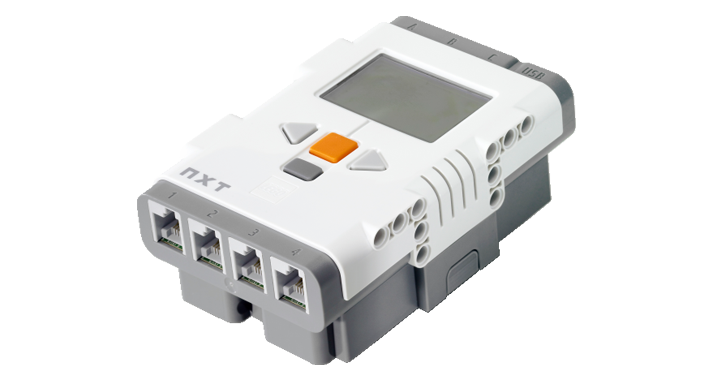
\includegraphics[width=0.5\textwidth]{Bilder/Robot/nxt_brick}
\caption{NXT-Stein}
\label{fig:nxtBrick}
\end{figure}

Der NXT-Stein bildet die Recheneinheit und damit die Hauptkomponente des NXT-Robotersystems. Er besitzt oben drei Ausgänge für Motoren über die gleichzeitig die Rotationssensoren in den Servo-Motoren ausgelesen werden.

Unten befinden sich vier Eingänge für verschiedene Sensoren, die je nach Anwendungszweck über Flachbandkabel bestückt werden können, etwa ein Licht-, Schall-, Tastsensor oder beliebige Kombinationen daraus. Dies macht das NXT-System zu einem sehr flexiblem da einfach konfigurierbaren Robotersystem.

Über einen USB-Anschluss oben wird der NXT mit dem PC verbunden um ihn mit Programmen zu versorgen. Hierfür wird von LEGO eine graphische Entwicklungsumgebung bereitgestellt um auch Neulingen den Einstieg in die Roboter-Programmierung zu vereinfachen und ihnen die Möglichkeit zu bieten schon innerhalb weniger Minuten einen funktionierenden Prototypen auf die Beine stellen zu können. Im Fall des CLEEN-R-Aufbaus wird jedoch lediglich die interne Bluetooth-Verbindung genutzt.

Vorne befindet sich ein 100 mal 64 Pixel auflösendes binäres LCD-Display über das Einstellungen getätigt oder Statusmeldungen ausgegeben werden können. Auch Sound-Ausgabe über einen integrierten 8-Bit-Lautsprecher ist möglich.

\subsection{Sensoren}

\subsubsection{Tastsensor}

\begin{figure}[h]
\centering
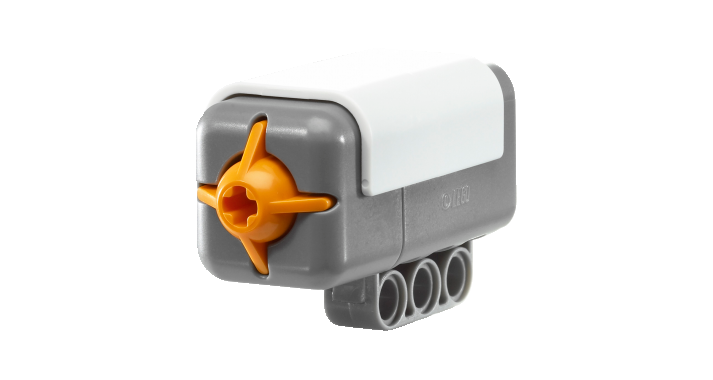
\includegraphics[width=\textwidth/3]{Bilder/Robot/button_sensor}
\caption{Tastsensor des NXT-Systems}
\label{fig:buttonSensor}
\end{figure}

Der berührungsempfindliche Sensor vorne diente zum Detektieren von Gegenständen im Bereich des Greifarms, woraufhin dieser geschlossen werden kann. Er wurde durch den Ultraschallsensor ersetzt, der nicht nur die unmittelbare Berührung bemerkt sondern auch ein herannahendes Objekt während der Fahrt detektiert.

\subsubsection{Rotationssensoren}

Die Rotationssensoren in den Servomotoren erlauben es dem NXT-Roboter, die Geschwindigkeit der Motoren abhängig des Widerstands (des Untergrunds) zu regulieren. So werden unter anderem präzises Abbremsen und Fehlerminimierung bei der Positionsbestimmung ermöglicht.

\subsubsection{Farbsensor}

\begin{figure}[h]
\centering
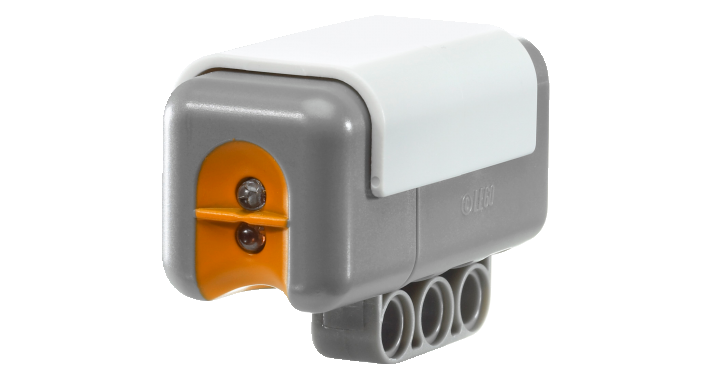
\includegraphics[width=\textwidth/3]{Bilder/Robot/color_sensor}
\caption{Farbsensor des NXT-Systems}
\label{fig:colorSensor}
\end{figure}

Der RGB-Sensor am Boden des NXT dient dazu, die Farbe des Bodens herauszufinden. Diese kann sowohl dazu genutzt werden, bei der Bildverarbeitung die Hintergrundfarbe herauszurechnen und so die Qualität der Objekterkennung zu erhöhen, als auch eine farblich markierte Zielzone im Raum finden zu können, auf der ein getragenes Objekt abgelegt werden kann.

\subsubsection{Ultraschallsensor}

\begin{figure}[h]
\centering
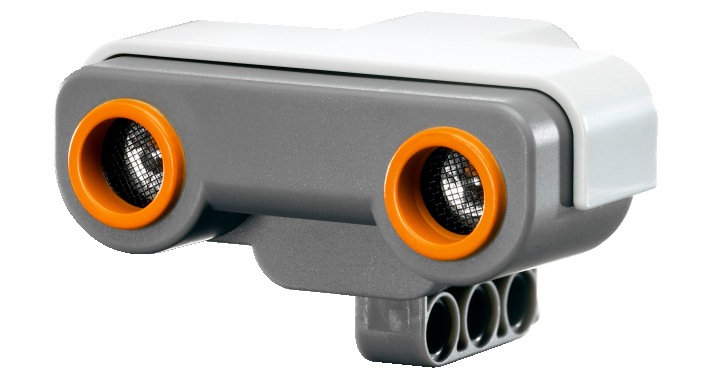
\includegraphics[width=\textwidth/3]{Bilder/Robot/distance_sensor}
\caption{Ultraschallsensor des NXT-Systems}
\label{fig:distanceSensor}
\end{figure}

Der Ultraschallsensor dient zur Messung der Distanz vom Roboter zum nächsten soliden Objekt. Hier wird er genutzt um zu detektieren, wie weit ein Objekt vom Greifarm entfernt ist, um diesen im geeigneten Moment zu schließen und so das Objekt mitnehmen zu können. Auch ermöglicht er ein geregeltes Heranfahren an ein Objekt. Die Präzision des Distanzsensors beträgt $\pm$3cm.

\subsection{Aktoren}

\subsubsection{Antriebsmotoren}

\begin{figure}[h]
\centering
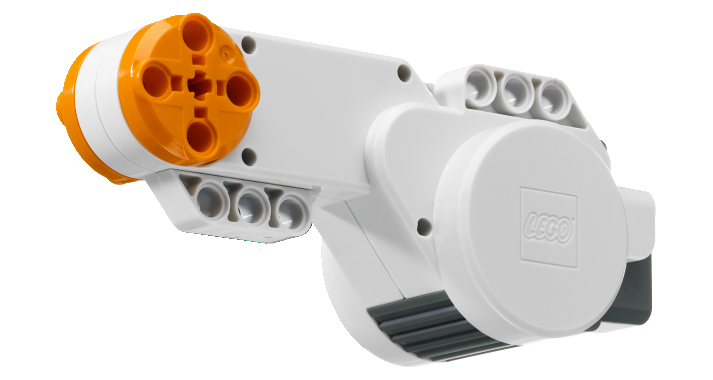
\includegraphics[width=\textwidth/3]{Bilder/Robot/motor}
\caption{Servo-Motor des NXT-Systems}
\label{fig:motor}
\end{figure}

Die beiden Servomotoren links und rechts des NXT-Roboters bilden den differentialen Antrieb und ermöglichen freie Fortbewegung.

\subsubsection{Greifarmmotor}
\label{greifarm}
Der dritte Motor im vorderen Teil des Roboters dient zum Öffnen und Schließen des Greifarms und so zur Mitführung von Gegenständen.

\section{Steuerung des Roboters}

Die Steuerung des Roboters durch das Smartphone erfolgt via Bluetooth.
Das Kommunikationsprotokoll und damit die nötigen Befehle zum Regeln der Aktoren und Auslesen der Sensoren wurde von LEGO dokumentiert und ist online erhältlich\cite{nxt_comm_protocol}.

\begin{figure}[h]
\centering
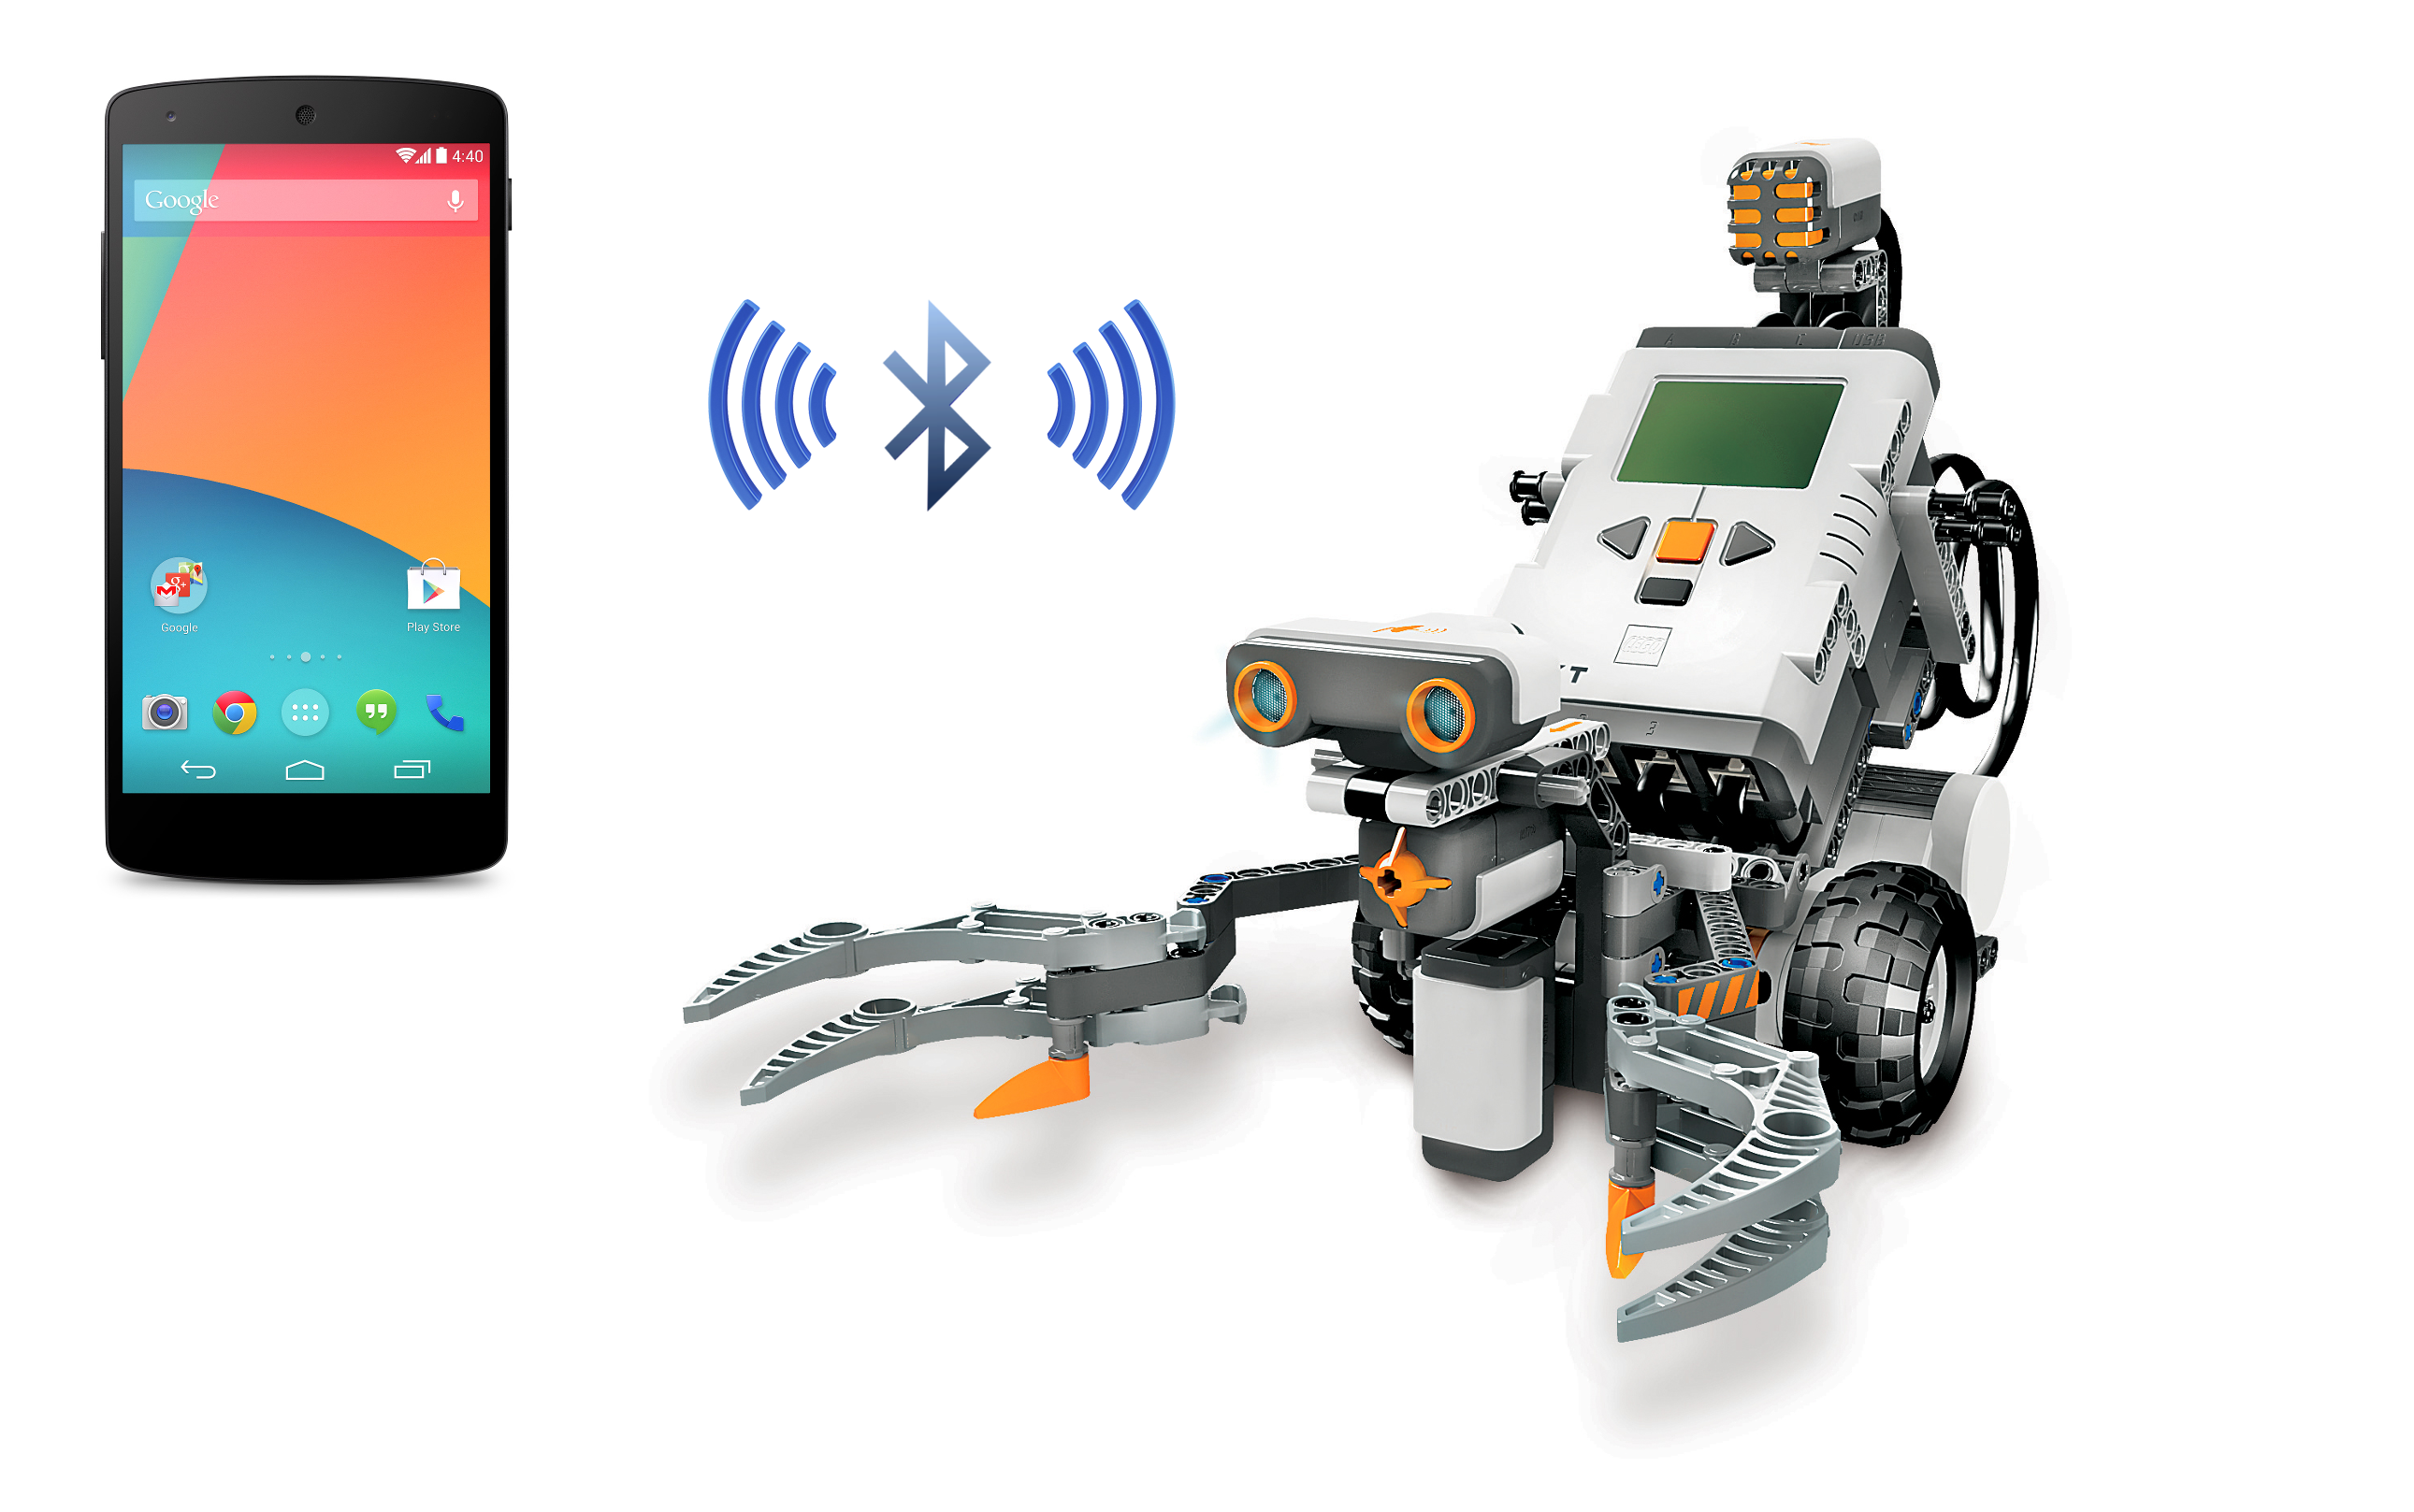
\includegraphics[width=\textwidth/2]{Bilder/Robot/bluetooth}
\caption{Bluetooth-Verbindung zwischen NXT und Nexus 5}
\label{fig:bluetooth}
\end{figure}

Auf dem NXT selbst wird hierbei kein Programm ausgeführt, um alle Logik zentral in der NXT-App auf dem Smartphone zu halten.

Zunächst muss eine Bluetooth-Verbindung erstellt werden, wozu beide Geräte aktiviertes Bluetooth aufweisen, der Roboter zusätzlich sichtbar für das Smartphone sein müssen.

Bei Erstverbindung muss der gesuchte NXT ausgewählt werden, danach ist die Bluetooth-Adresse bekannt und die App kann ohne Benutzerinteraktion eine Verbindung mit dem NXT-Roboter aufnehmen.

Kommt eine Verbindung zustande, können seriell Byte für Byte die Kommandos an den NXT übertragen, eventuelle Antworten empfangen werden.

App-seitig übernimmt ein gesonderter Thread in der Klasse NxtTalker nach Zustandekommen einer Verbindung das Management der Daten.

Zum Bewegen der Motoren muss zunächst per Befehl pro Aktor eine Geschwindigkeit (und Parameter wie Regulierung) übergeben, zum Stoppen können alle Motoren mit einem Befehl auf Geschwindigkeit '0' gesetzt werden.

Zwei Motoren können synchronisiert werden, sodass diese gleichzeitig starten. Ansonsten würde der Zeitversatz zwischen dem Absetzen der zwei 'setze Geschwindigkeit'-Befehle bewirken, dass der Roboter vor dem geradeaus fahren kurz nur das erste Rad ansteuert und in eine Richtung abdriftet.

\section{Wahl des Kameramoduls}
\label{sec:Kamera}

Die Hauptfrage bezüglich des Kameramoduls bestand in der Wahl zwischen einem Ein- oder einem Zweikamerasystem.

Der Vorteil eines Zweikamerasystems besteht in der Möglichkeit für wesentlich bessere Orientierung im 3D-Raum, da Entfernungen mittels der beiden Differenzbilder präziser berechnet werden können.
Im Gegensatz dazu ist beim Einkamerasystem die Entfernungsberechnung auf ein 2D-Bild beschränkt und nicht annähernd so genau.

Jedoch ist der Berechnungsaufwand für das Auswerten zweier Differenzbilder ungleich höher, weshalb sich letztendlich aufgrund dieser Ungleichheit des Implementierungsaufwandes für ein Einkamerasystem entschieden werden.

Weitere Aspekte sind Auflösung und Öffnungswinkel des Kameramoduls.
Höhere Auflösung bedeutet bessere Erkennung von Gegenständen auf weitere Entfernungen; Ein größerer Öffnungswinkel heißt, dass mehr Raum in einem Bild erfasst werden kann, somit weniger Drehbewegung des Roboters in Richtung eines Objekts nötig ist, bis es erfasst und detektiert werden kann.

Ein Problem bei der Kamera des Nexus ist, das sich diese nicht zentral auf dem Rücken des Smartphones befindet, sondern nach links oben versetzt. Dies setzt voraus, dass entweder Software- oder Hardwareseitig dieser Versatz aus der Bildverarbeitung kompensiert wird.

Hier wurde der Einfachheit halber die Halterung am Roboter verschoben, wodurch aus der Sicht des Roboters die Kamera in der Mitte liegt.

\begin{figure}[h]
\centering
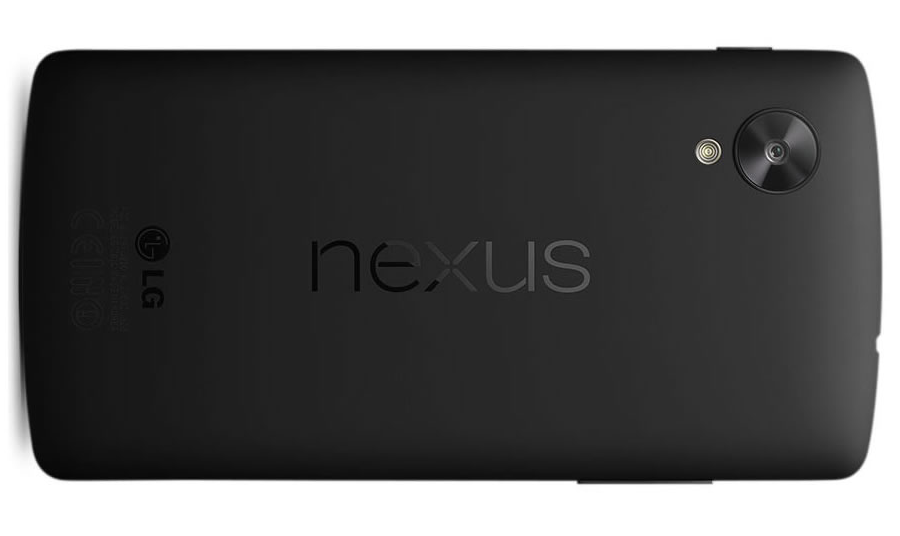
\includegraphics[width=\textwidth/3]{Bilder/Robot/nexus_backside}
\caption{Kameramodul des Nexus 5}
\label{fig:camera}
\end{figure}


\chapter{Softwareumsetzung}
\label{cha:Software}

Mit Hilfe des in Kapitel \ref{sec:Kamera} beschriebenen Kameramoduls müssen verschiedene Aufgaben aus dem Bereich der Bildverarbeitung bewältigt werden. 

\section{Wahl der Bildverarbeitungsbibliothek}

Die Umsetzung der zu bewältigenden Aufgaben kann durch die Wahl einer geeigneten Bildverarbeitungsbibliothek deutlich vereinfacht werden. Wichtige Kriterien für die Wahl der Bibliothek sind unter anderem Funktionsumfang, Dokumentation und Aktivität der Community.

\subsection{LibCCV}

LibCCV \cite{libccv} ist eine open-source Bildverarbeitungsbibliothek, die viele bekannte Algorithmen implementiert. LibCCV steht unter einer BSD-Clause-3-Lizenz und kann somit für eine Studienarbeit problemlos unbegrenzt verwendet werden. Die Bibliothek ist größtenteils in C++ verfasst und somit potenziell auf einem Android-Smartphone verwendet werden. Die Verwendung auf dem Smartphone wird jedoch nicht offiziell unterstützt und kann potenziell weitere Schwierigkeiten mit sich bringen.

\subsection{Imagemagick}

Bei Imagemagick \cite{imagemagick} handelt es sich um eine Bildverarbeitungsbibliothek, welche sehr viele Algorithmen bereits implementiert hat. Algorithmen zur Objekterkennung müssten jedoch vollständig selbst implementiert werden, was zu einem großen zusätzlichen Aufwand führen kann. Imagemagick wird unter der Apache 2.0 Lizenz vertrieben.

\subsection{OpenCV}
\label{subsec:opencv}

OpenCV \cite{opencv_library, bradski2008learning} stellt eine der größten Open-Source-Bibliotheken für Bildverarbeitung da. Die Bibliothek hat einen starken Fokus auf Echtzeitverarbeitung und wird daher auch in vielen Projekten im Bereich der Robotik verwendet. OpenCV hat eine große aktive Community, wodurch eventuelle Fragen und Probleme schnell beantwortet werden können. Zusätzlich bietet OpenCV eine offizielle Version für Android und eignet sich somit ideal für diese Studienarbeit.


\section{Algorithmen zur Objekterkennung}
\label{sec:Objekterkennung}

Aufgabe des Roboters, ist es Gegenstände in einem Raum mit Hilfe von Kamerabildern zu erkennen. Folglich spielt die Objekterkennung eine große Rolle.

\subsection{Farbbasierte Objekterkennung}
Einen einfachen Ansatz der Objekterkennung unter Verwendung von Methoden der in \ref{subsec:opencv} beschriebenen Bibliothek OpenCV stellt eine farbbasierte Objekterkennung dar. Hierfür wird das Kamerabild zunächst vom RGB-Format in das HSV-Format konvertiert. Dies wird durchgeführt, da das HSV-Format unempfindlicher gegen Veränderungen in der Beleuchtung ist als das RGB-Format \cite{cucchiara2001improving}. Abbildung \ref{fig:ColorModels} zeigt die Aufteilung eines Bildes in die verschiedenen Kanäle.

\begin{figure}[h]
\centering
\includegraphics[width=\textwidth]{Bilder/Software/ColormodelsAll}
\caption{Beispiel einer Aufspaltung in RGB-Kanäle (links) und HSV-Kanäle (rechts)}
\label{fig:ColorModels}
\end{figure}

Wie in Abbildung \ref{fig:ColorModels} zu sehen ist, eignet sich vor allem der Saturation-Kanal des Bildes um farbige Objekte zu erkennen, da dieser hohe Werte annimmt wenn die Farbintensität hoch ist. Zuletzt erfolgt eine Binarisierung mit einem empirisch ermittelten Schwellwert von 50. Dies ist notwendig, da die, in der OpenCV-Bibliothek implementierte, Methode von Suzuki und Abe \cite{suzuki1985topological} zur Segmentierung von Objekten ein Binärbild erwartet. Aus dem in Abbildung \ref{fig:ColorModels} dargestellten Beispiel entsteht nach der Binarisierung schließlich Abbildung \ref{fig:BinarizedColorModels}. Der Algorithmus zur Segmentierung erkennt daraus drei Objekte und zeichnet ihren Konturen, wie in Abbildung \ref{fig:SegmentedColorModels} ersichtlich, ein.

\begin{figure}[h]
\centering

\includegraphics[width=\textwidth/2]{Bilder/Software/ColormodelsBinarized}
\caption{Beispiel der Binarisierung des Sättigungskanals}
\label{fig:BinarizedColorModels}
\end{figure}
\begin{figure}[h]
\centering
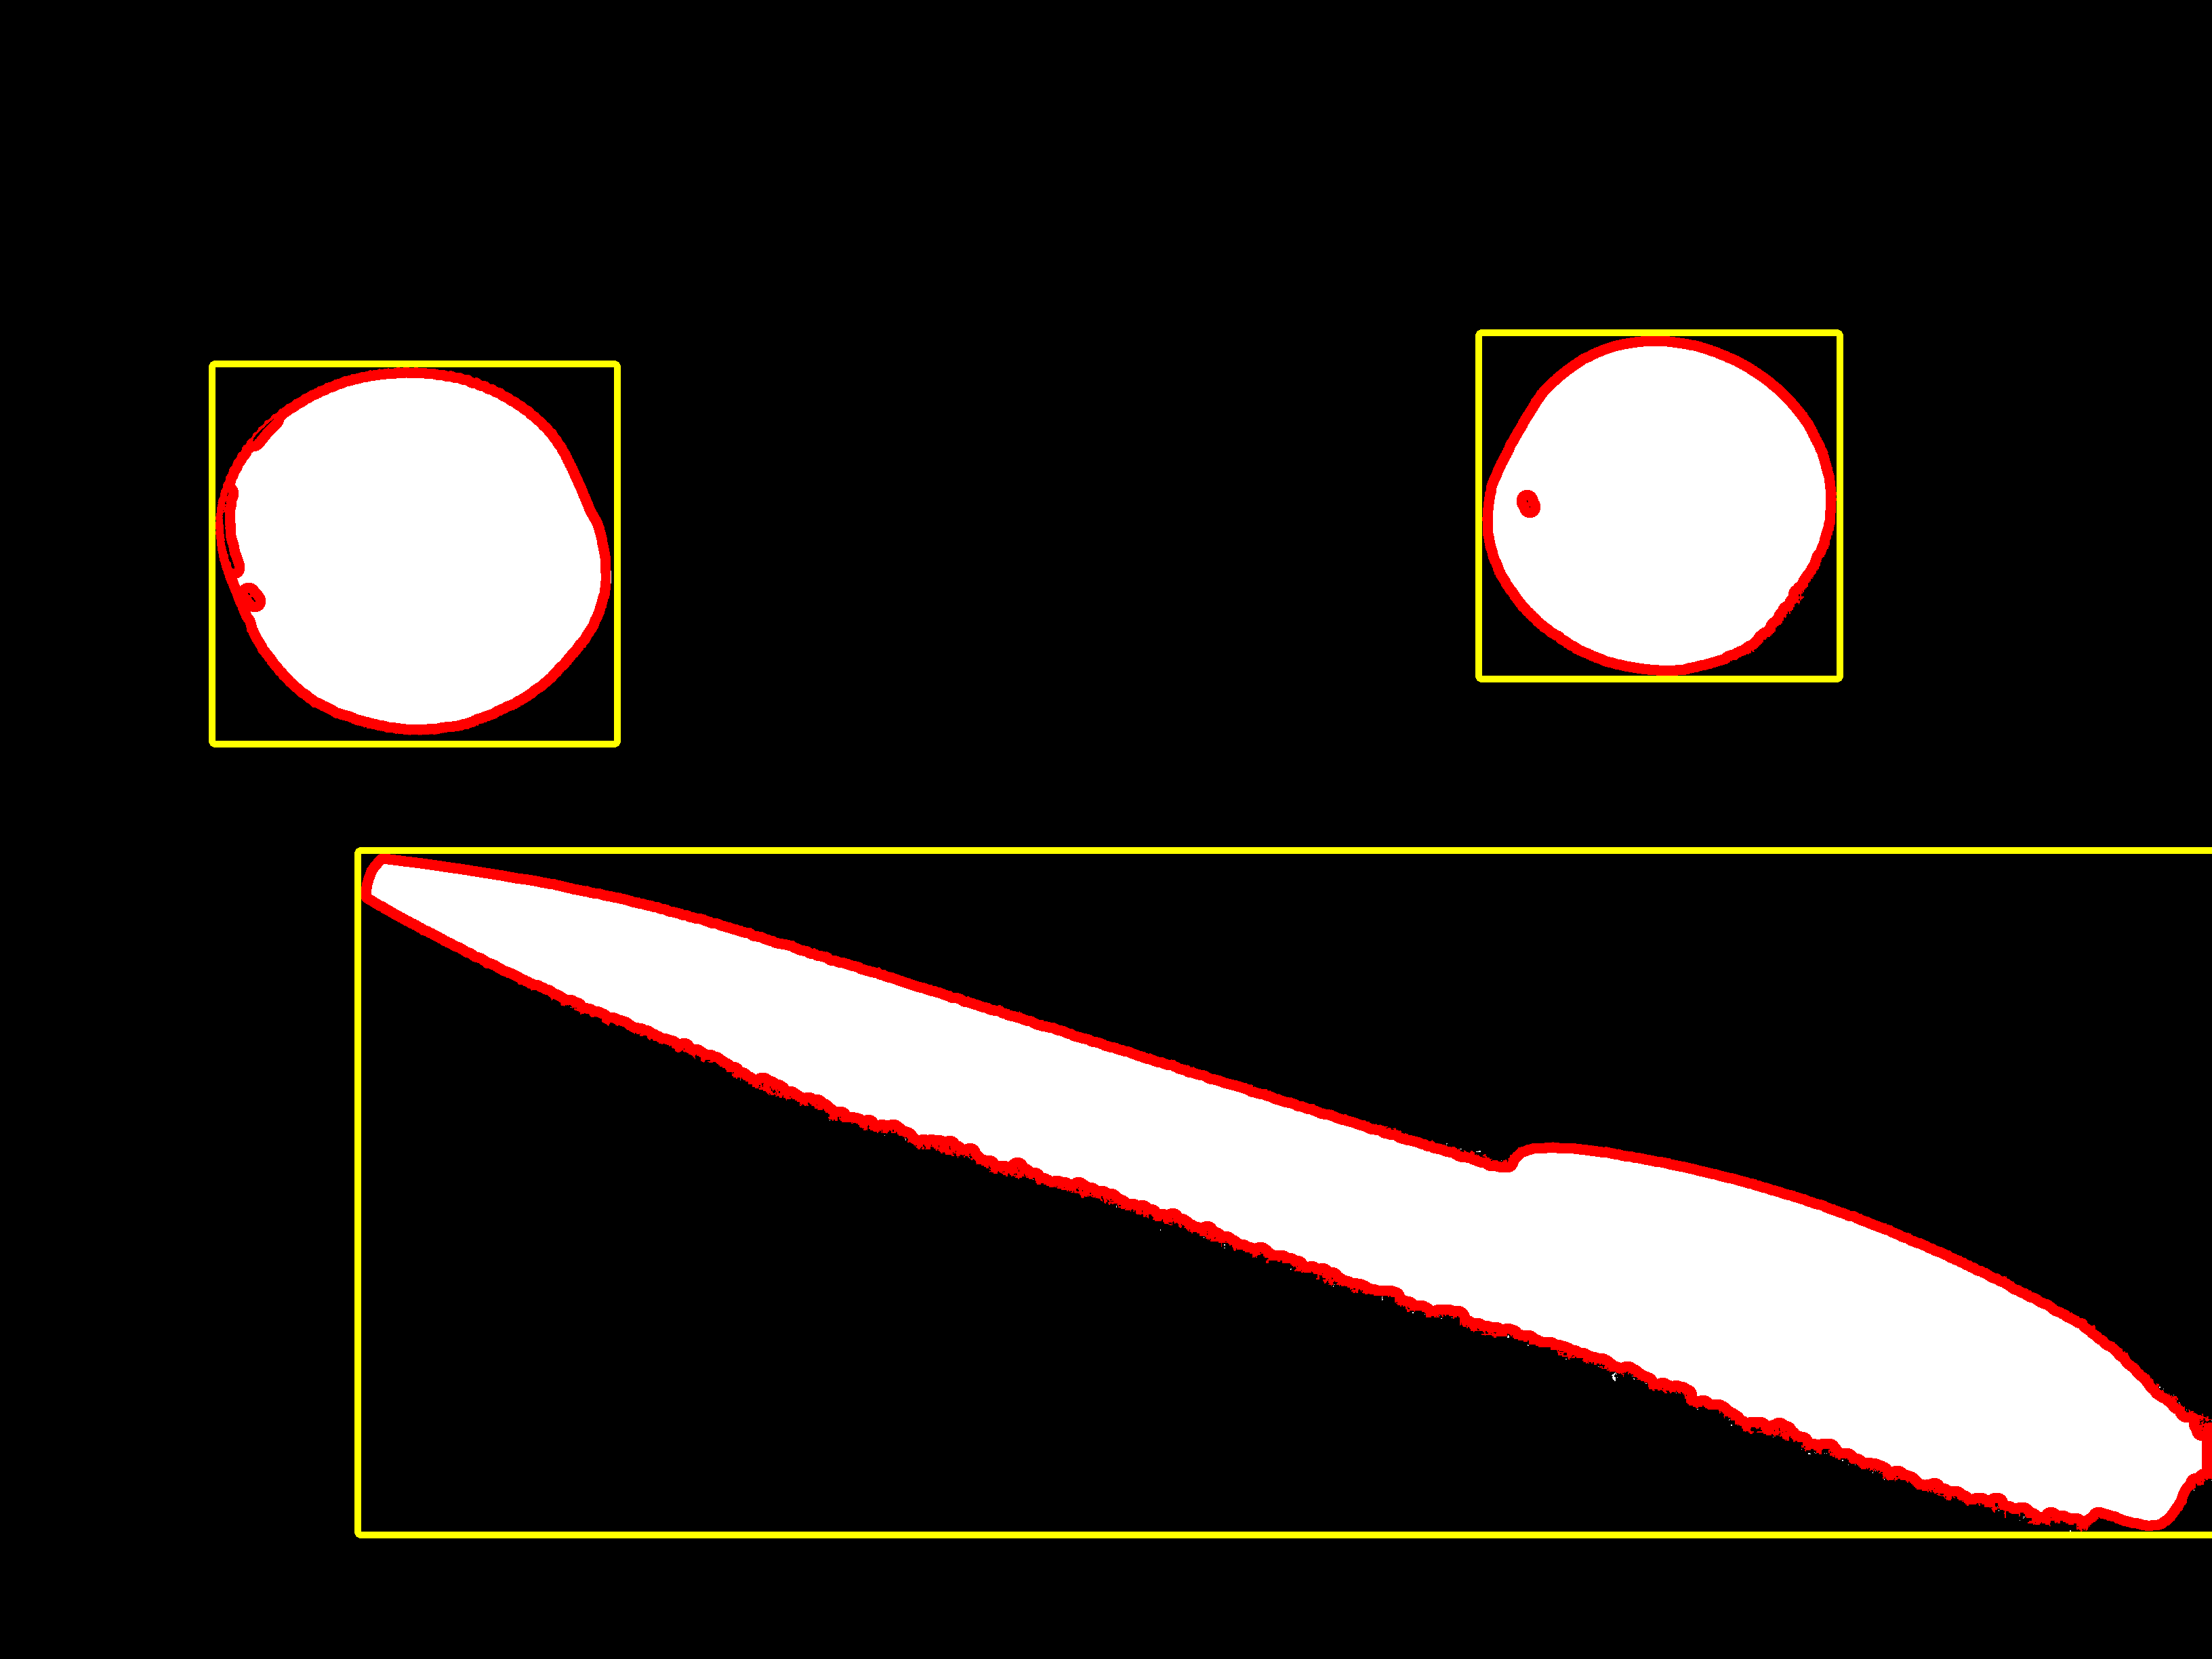
\includegraphics[width=\textwidth/2]{Bilder/Software/ColormodelsSegmentated}
\caption{Beispiel einer Segmentierung des binarisierten Sättigungskanals}
\label{fig:SegmentedColorModels}
\end{figure}

\section{Ortsbestimmung}
\label{sec:Ortsbestimmung}

Die Aufgabe des Roboters ist es, Gegenstände in vordefinierte Bereiche zu befördern. Hierzu muss ihm jederzeit bekannt sein wo diese sich befinden, bzw. wo er sich relativ zu diesen aufhält, um sie anfahren zu können.

\subsection{Mitteilung von Beobachterkomponente}

Ist im Raum ein weiteres System vorhanden, dessen Position konstant und dem Roboter zu jedem Zeitpunkt bekannt ist, kann eine simple, und genaue Positionsbestimmung erfolgen. Eine solche Beobachterkomponente kann über Sensordaten, wie beispielsweise einer Kamera oder einem Ultraschallsensor, zu jedem Zeitpunkt Kontakt zu Roboter haben.
Der Roboter muss hierbei keine Berechnungen durchführen und verlässt sich für die korrekte Positionsbestimmung auf den Beobachter, von welchem zu jedem Zeitpunkt Position und Orientierung des Roboters im Raum abrufbar ist.

Die Beobachterkomponente stellt eine sehr effiziente Art von Ortsbestimmung dar, hat jedoch den beträchtlichen Nachteil, dass zusätzliche Hardware erforderlich ist.

\subsection{Raumanalyse}

Bei der Raumanalyse werden Kamerabilder analysiert und aus ihnen Fixpunkte oder Geraden extrahiert, mit denen sich der Roboter bei Bewegung im Raum zu orientieren versucht. Dies ist ein sehr rechenaufwändiges Verfahren, welches zusätzlich mit einer großen Implementierungsarbeit verbunden ist.

Zusätzlich stellt dieses Verfahren Anforderungen an den Raum in dem es verwendet wird. Im Raum müssen genügend charakteristische Orientierungspunkte vorhanden sein. Verliert der Roboter die Orientierung, ist es nicht ohne weiteres möglich diese wiederzuerlangen.

Vorteil des Verfahrens der Raumanalyse ist, dass die benötigte Hardware in Form eines Kameramoduls und eines leistungsstarken Prozessors bereits vorhanden ist.

\subsection{Positionsverfolgung}

Die Positionsverfolgung als Mittel der Ortsbestimmung bietet sich bei Robotern an, welche einen sehr exakten Sensor zur Beobachtung der zurückgelegten Strecke besitzen. Über die zurückgelegte Strecke und die Orientierung des Roboters kann zu jedem Zeitpunkt ein Bewegungsvektor erzeugt werden, der die genaue Position des Roboters bestimmt.

Problematisch bei diesem Verfahren ist jedoch, dass eine sehr genaue Bestimmung der zurückgelegten Strecke benötigt wird. Fehler bei der Bestimmung wirken sich additiv aus. Die hat zur Folge, dass die Positionsverfolgung bei längeren Fahrten immer ungenauer wird. Eine Art der Streckenbestimmung stellen beispielsweise Rotationssensoren in Rädern dar. Hierbei wird die Genauigkeit des Verfahrens durch das Spiel der Räder und der Auflösung der Sensoren beeinträchtigt.

Da das CLEEN-R-Projekt nicht über die zusätzliche Hardware einer Beobachterkomponenten verfügt und der zusätzliche Aufwand der Auswertung der Kamerabilder zur Merkmalsextraktion zu aufwändig wäre, wurde sich für die Variante der Positionsverfolgung entschieden. Die Auflösung der Rotationssensoren ist mit 1\degree\ ausreichend genau. Die automatische Geschwindigkeitsanpassung der NXT-Motoren abhängig des Untergrunds fördern zusätzlich eine exakte Ortsbestimmung über die Positionsverfolgung.

\section{Struktur der Applikation}
Da es sich um eine große Applikation mit mehr als 3000 Zeilen Code und 33 Klassen handelt, sind in den folgenden Abschnitten lediglich Kernelemente herausgegriffen und im Detail erklärt.

\subsection{Grundstruktur}
Eine Android Applikation muss mindestens eine Klasse haben, die von der abstrakten Klasse \textit{Activity} erbt. Diese Activity, oftmals \textit{MainActivity} genannt, wird beim Starten der Applikation aufgerufen. Sie verwaltet grafische Oberflächen, sowie das Verhalten der Applikation beim Starten, Schließen oder Pausieren. Im CLEEN-R-Projekt stellt die \textit{MainActivity} zusätzlich eine Schnittstelle zur OpenCV-Bibliothek dar. Die Activity wird über eingehende Kamerabilder informiert und vermittelt diese weiter an den Controller der Applikation; die Klasse \textit{CleenrBrain}.

Zusätzlich hält die \textit{MainActivity} eine Referenz zur Klasse der Hardwareansteuerung \textit{NxtTalker}. Abbildung \ref{fig:UMLActivity} zeigt die Grundstruktur der \textit{MainActivity}

\begin{figure}[h]
\centering
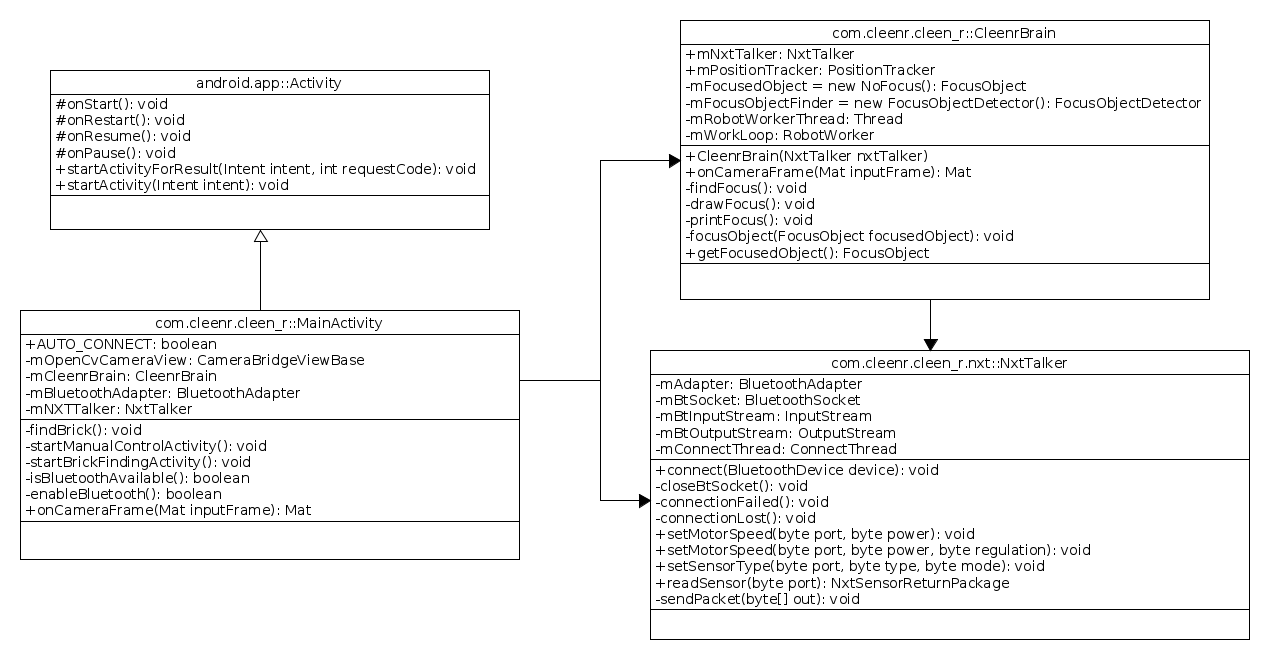
\includegraphics[width=\textwidth]{Bilder/Software/UML/MainActivity}
\caption{UML-Klassendiagramm der Grundstruktur der Applikation}
\label{fig:UMLActivity}
\end{figure}

 
\subsection{Fokusobjektfindung}

Die Controllerklasse \textit{CleenrBrain} hat die Aufgabe den Roboter zu koordinieren. \textit{CleenrBrain} hält eine Referenz zu einem \textit{FocusObject}-Objekt, welches den aktuell fokussierten Gegenstand repräsentiert. Hierbei wird auch das Fehlen eines Fokusobjekts aus Gründen der Polymorphie als Objekt beschrieben. \textit{CleenrBrain} wird beim vorliegen einer neuen Kameraaufnahme benachrichtigt und ermittelt daraufhin mit Hilfe einer \textit{FocusObjectDetector}-Klasse ein neues \textit{FocusObject}. Hierbei wird, wie in Kapitel \ref{subsec:Auffindung} beschrieben versucht einen Gegenstand über mehrere Aufnahmen hinweg im Fokus zu behalten. Abbildung \ref{fig:UMLFocus} beschreibt das Zusammenspiel der beschriebenen Klassen anschaulich.

\begin{figure}[h]
\centering
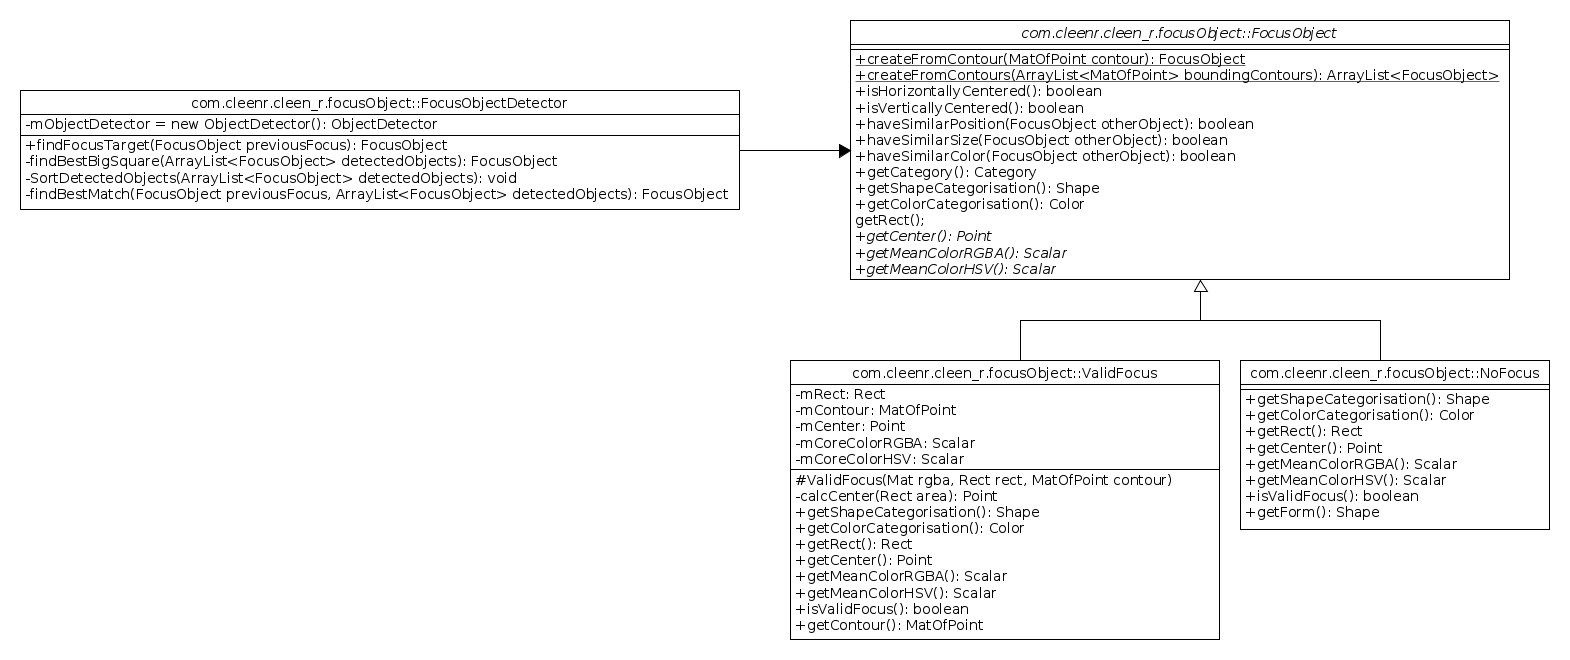
\includegraphics[width=\textwidth]{Bilder/Software/UML/FocusObjects}
\caption{UML-Klassendiagramm der für die Auffindung eines Fokusobjekts verantwortlichen Klassen}
\label{fig:UMLFocus}
\end{figure}

\subsection{Objektkategorisierung}

Wie auch aus Abbildung \ref{fig:UMLFocus} ersichtlich, beinhaltet die \textit{FocusObject}-Klasse eine Methode zur Kategorisierung des Gegenstands. Hierbei wird eine Kategorie der Klasse \textit{Category} erzeugt, welche sich aus den beiden Feldern \textit{Color} und \textit{Shape} zusammensetzt.

\begin{figure}[h]
\centering
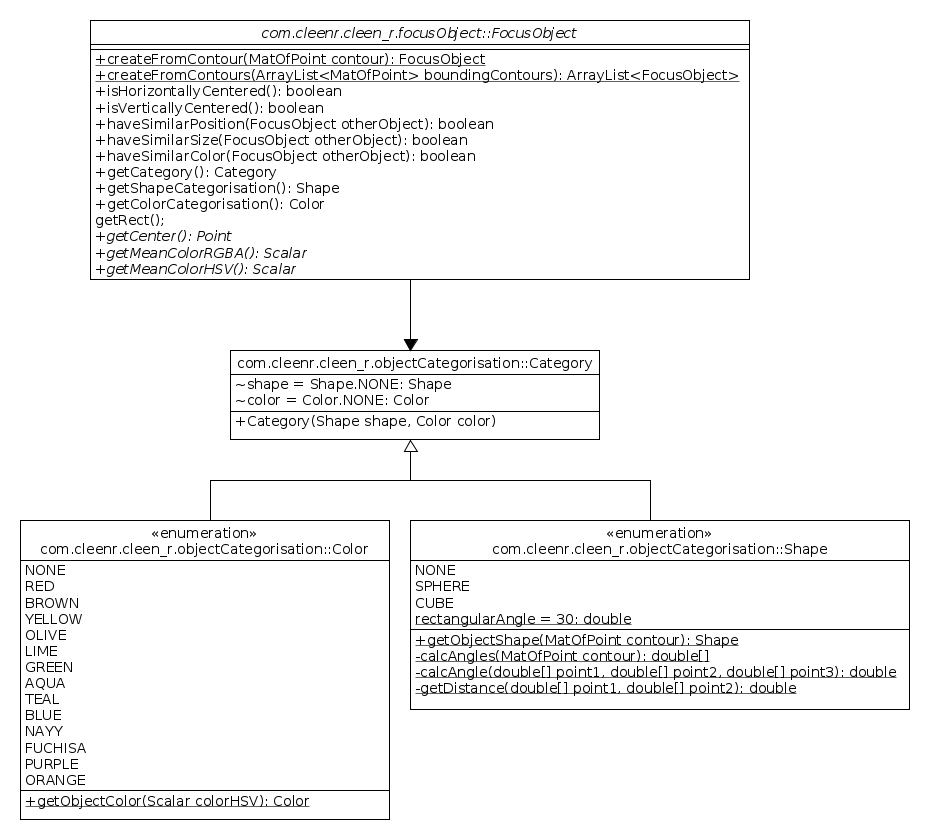
\includegraphics[width=\textwidth]{Bilder/Software/UML/Categories}
\caption{UML-Klassendiagramm der Kategorisierung von Fokus Objekten}
\label{fig:UMLCategorisation}
\end{figure}

\subsection{Positionsdetektion}

\subsection{Bluetooth-Verbindung}

\subsection{Arbeitsphasen}

Die Controllerklasse \textit{CleenrBrain} verwaltet mit Hilfe eines zusätzlichen Threads den Arbeitszyklus des Roboters. Durch die Verwendung eines zweiten Threads kann die Suche nach neuen Fokus Objekten in folgenden Aufnahmen parallel zur Abarbeitung der in Kapitel \ref{cha:Workloop} beschriebenen Arbeitsphasen geschehen. 

Die Arbeitsphasen sind separat als eigene Klassen modelliert, die sich von einer abstrakten Klasse \textit{WorkPhase} ableiten. Jede Arbeitsphase verfügt über eine virtuelle \textit{executeWork}-Methode, welche Zugriff auf alle für die Arbeitsphase relevanten Operationen besitzt. Darunter zählen Steuerwerk des Roboters, eine Referenz auf das aktuelle Fokusobjekt und einer Möglichkeit die Arbeitsphase zu wechseln. Die Implementierung der \textit{PickingUpObject}-Klasse ist in Listing \ref{lst:Pickup} erkennbar. Es ist deutlich zu sehen, dass der Code durch die hinzugefügte Abstraktionsebene sehr einfach gehalten werden kann.

\begin{lstlisting}[caption={Implementierung der Arbeitsphase \glqq Gegenstand aufnehmen\grqq }, label=lst:Pickup]
public class PickingUpObject extends WorkPhase {
    public PickingUpObject(RobotWorker worker) {
        super(worker);
    }
    @Override
    public void executeWork(FocusObject focusObject, RobotControlUnit controlUnit) {
        controlUnit.closeClaw();
        if (!controlUnit.hasObjectInClaw()) {
            controlUnit.openClaw();
            mRobotWorker.switchWorkphase(new SearchingObject(mRobotWorker));
            return;
        }
        mRobotWorker.switchWorkphase(new CategorisingObject(mRobotWorker));
    }
}
\end{lstlisting}


\chapter{Tests des Robotersystems}
\label{cha:tests}
\section{Tests im gesicherten Rahmen}

\section{Realtests}
\chapter{Zusammenfassung und Ausblick}
\label{cha:Fazit}

Im Rahmen dieser Studienarbeit wurde das Robotersystem CLEEN-R entwickelt. Ziel war es mit Hilfe eines LEGO\textregistered\ Mindstorm NXT-Robotersets und eines Google Nexus 5 Android Smartphone ein Robotersystem zu entwickeln, welches kameragestützt Objekte erkennen, kategorisieren und transportieren sollte. 

In den vorhergehenden Kapiteln wurde zunächst die \hyperref[cha:Materials]{konkrete Anwendung der Hardware}  beschrieben. Daraufhin ist die \hyperref[cha:robot]{Konstruktion des Roboters} geschildert. In den darauf folgenden Kapiteln sind \hyperref[cha:Software]{genaue Algorithmen zur Bildverarbeitung}, sowie der \hyperref[cha:Workloop]{allgemeine Arbeitszyklus} des Systems beschrieben. Zuletzt folgen \hyperref[cha:Tests]{Tests in geschützten Raum, sowie Realtests}.

\section{Zusammenfassung}

Wie aus Kapitel \ref{cha:Tests} ersichtlich, konnte ein Robotersystem konstruiert werden, welches erfolgreich Gegenstände \glqq aufräumen\grqq\ kann. Das System besteht aus zwei getrennten Modulen: Ein LEGO Mindstorm NXT-Roboter und ein Google Nexus 5 Android-Smartphone kommunizieren über eine Bluetooth-Schnittstelle mit einander und steuern so die Aktoren des Roboters. 

Es konnte ein Großteil der Komplexität des Systems dadurch reduziert werden, dass das Smartphone als zentrale Steuereinheit benutzt wird und das NXT-System lediglich als Vermittler zu Sensoren und Aktoren genutzt wird. Der Roboter basiert auf einem modifizierten Bauplan, der von LEGO zur Verfügung gestellt wurde. Dieser Bauplan wurde dahingehend angepasst, dass einige Sensoren entfernt und durch eine Halterung für das Smartphone ersetzt wurden.

Die Implementierung erfolgte mit der OpenCV-Bibliothek in einer Android-Applikation. Hierbei wurden verschiedene Verfahren der Bildverarbeitung eingesetzt um Objekte zu erkennen. Konkret wird in den Kameraaufnahmen nach Objekten mit hoher Farbsättigung gesucht. Bilder werden anschließend binarisiert und mit Hilfe von Algorithmen zur Kantenverfolgung segmentiert. 

Ist ein Objekt erkannt, so fährt der Roboter es an und nimmt es mit einem Greifarm auf. Das Ansteuern des Objekts geschieht hierbei mit einer Kombination aus Sensordaten aus einem Ultraschallsensor und der Kamera des Smartphones. Wenn das Objekt erfolgreich aufgenommen wurde, wird es auf Grund seiner Farbe und Form kategorisiert. Je nach Kategorie, wird eine andere Zielzone ausgesucht und lokalisiert.

Ist eine Zielzone bestimmt worden, transportiert der Roboter den aufgenommenen Gegenstand dort hin und legt ihn ab. Anschließend begibt er sich zurück in die Startposition und beginnt die Suche von vorne. Die Orientierung im Raum wurde dabei über einen Positionsverfolgungsansatz gelöst, welcher die gefahrene Strecke berechnet um die aktuelle Position zu bestimmen.

\section{Bewertung der Ergebnisse}

Die Hauptaufgabe wurde erfolgreich gelöst. Es wurde ein Robotersystem entwickelt, welches alle in der \hyperref[cha:Problemstellung]{Problemstellung} beschriebenen Aufgaben erfolgreich Lösen kann. 

Bei der Entwicklung traten an vielen Stellen, wie beispielsweise der in Kapitel \ref{subsec:Entfernungsschätzung} beschriebenen Entfernungsschätzung, schwierige Probleme auf, welche durch zum Teil sehr elegante Lösungswege gelöst werden konnten. Es wurden stets mehrere Möglichkeiten abgewägt, wobei sich an einigen Stellen gezeigt hat, dass zusätzliche Hardware eine elegantere Lösung darstellt. Es ist jedoch auch zu beachten, dass diese immer einen zusätzlichen Entwicklungsaufwand mit sich führt und zusätzliche Mittel in Anspruch nimmt, die bei einem kleineren Roboterprojekt oft nicht vorhanden sind. 

Wie Kapitel \ref{cha:Tests} zeigt, funktioniert die Koppelung des Smartphones als Kameramodul mit dem NXT-Roboter. Die zentrale Designentscheidung das Smartphone als Steuereinheit zu benutzen und den Roboter lediglich ausführende Tätigkeiten verrichten zu lassen hat sich als sehr gewinnbringend herausgestellt. Durch die geringe Rechenleistung des NXT-Steins wäre eine effiziente Berechnung von Algorithmen der Bildverarbeitung nicht möglich gewesen.

Über das Verhalten des Roboters lässt sich sagen, dass es noch sehr abgehackt wirkt. Bewegungen sind nicht flüssig, Drehungen oft langsam und das Positionstracking manchmal ungenau. All diese Einflüsse erwecken den Eindruck der Roboter sei unfertig. In nachfolgenden Abschnitt wird ein Ausblick über weitere Vorgehensweisen bei der Bearbeitung dieser Themen gewährt.

\section{Ausblick}

Ein Hauptproblem des aktuellen Robotersystems stellt das \glqq abgehackte\grqq\ Fahren dar. Der Roboter fährt nie eine Kurve, sondern hält an und dreht sich auf der Stelle. Dies erleichtert das Positionstracking und das Zentrieren von Objekten ohne das Risiko sie zu Überfahren, ist jedoch zeitlich ineffizient und wird von Beobachtern als \glqq unschön\grqq\ empfunden. Ein flüssigeres Verhalten kann durch den ausgefeilteren Einsatz des Ultraschallsensors erreicht werden. Hierbei kann die Geschwindigkeit des Heranfahrens an ein Objekt an die gemessene Entfernung angepasst werden.

Eine weitere Möglichkeit der Erweiterung des Systems stellt die Verwendung einer zweiten Kamera dar. Diese zweite Kamera kann zwei mögliche Anwendungen haben. Sie könnte als zusätzliches Kameramodul auf dem Roboter Tiefeninformationen aus Bildern erzeugen und so eine Kartografierung der Umgebung beginnen. Der Roboter könnte so als lernendes System Räume einstudieren und zu transportierende Gegenstände als \glqq Fremdkörper\grqq\ im Raum identifizieren. Alternativ könnte eine zweite Kamera als externer Beobachter des Systems verwendet werden. Dies würde wie in Kapitel \ref{subsec:Beobachter} beschrieben zu einer genaueren Positionserkennung beitragen und das System somit stabiler gegen Ungenauigkeiten der Rotationssensoren machen.

Insgesamt lässt sich sagen, dass noch einige offene Nahtstellen im Projekt vorhanden sind, an denen zukünftige Entwickler Erweiterungen und Verfeinerungen anbringen können. Durch die modulare Struktur der Applikation lässt sich nahezu der gesamte Code ohne große Änderungen für weitere Projekte benutzen.

\section{Reflexion des Gelernten}

	}{}
	
	\ifthenelse{\boolean{RomanNumbering}}
	{
		\pagenumbering{Roman} 
		\setcounter{page}{\romannumber}
	}{}
	
	
	\ifthenelse{\boolean{Literaturverzeichnis}}
	{
		\bibliographystyle{unsrt}
%\bibliographystyle{alphadin}
\bibliography{Dependencies/quellen}	
	}{}
	
	

\end {document}
